% Sune
%TODO:
% Apply defintiions
% Short introduction to Architecture qualities
As software engineers our focus is on creating a software architecture based on the architectural requirements. Software architecture allows us to reasons and take qualified decision. It is essential that we early in the project    \cite{un}

\section{Quality Attributes}
We will follow the definition on software architecture from \cite{Bass}. 
%**************************************Definition Software architecture
\begin{defi}[\textbf{Software architecture}]
The software architecture of a system is the set of \textbf{structures} needed to reason about the system, which comprise software \textbf{elements}, \textbf{relations} among them, and the \textbf{properties} of both. 
\end{defi}
%**************************************Definition Software architecture End


Our approach towards implementing a software architecture is based on Quality attribute (QA) and Quality attribute scenario (QAS). A quality attribute (QA) according to \cite{Bass} is as follows.

%**************************************Definition Quality attribute
\begin{defi}[\textbf{Quality attribute}]
..A quality attribute is a measurable or testable property of a system that is used to indicate how well the satisfies the needs of its stakeholders..  
\end{defi}
%**************************************Definition Quality attribute End


% TODO:
% Introduction to QA
% List relevant quality attributes
% Why these attributes?
% Relate to generel mobile application challenges and tactics

From \cite{Bass} we have seven quality attributes here among modifiability, availability and performance. Furthermore \cite{Kjaergaard:2015:AQT:2737182.2737196} has added energy efficiency and and ressources adaptability.  


We will discuss different tactics on software architecture for achieving the business goal for the electronic voting application. A tactic according to \cite{Bass} is defined as.

%**************************************Definition Tactic
\begin{defi}[\textbf{Tactic}]
Tactic is a design decision that influences the achievement of a quality attribute response. 
\end{defi}
%**************************************Definition Tactic End

\section{Quality Attribute Scenarios}
% TODO:
% Formal definition of QAS
% Use template from Bass

A core observation is that a QA should be measurable or testable quality. The key point is when working with QA we use them in a given context/scenario and therefor we informally call these as QAS.\\



\begin{figure}[H]
\centering
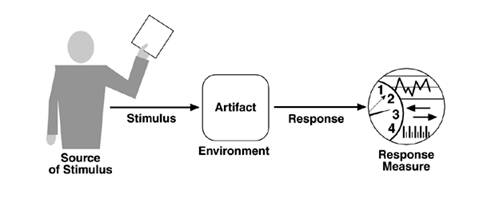
\includegraphics[scale=0.8]{QualityAttributeScenario.jpg}

\caption{The parts of a quality attribute scenario}
\label{fig:Quality_Attribute_Scenario}
\end{figure}






One of the core aspects of the definition of software architecture, is that software architecture is a set of structures, which we can use to reason about the system. To assist and visualize these structures, elements, relations and properties we use Module-, Component \& Connector (C\&C)- and Allocation viewpoints \cite{3+1}. 

\begin{enumerate}
    \item Module viewpoint is concerned with how functionality of the system maps to static development units. The focus will be on elements such as classes and interfaces and relationships such as associations, generalizations, realizations and dependencies.
    \item Component \& Connector viewpoint is concerned with the runtime mapping of functionality to components of the architecture. Components are the executing things that perform a function. Connectors are the communication channels between components. The purpose is to focus on the flow of data and responsibilities such as a network call or method call etc.
    \item Allocation viewpoint is concerned with how software entities are mapped to environmental entities. Here the focus are on the physical stuff such as computer or a network. We specify the environment in order to make the software running. 
\end{enumerate}


These viewpoint originates from $3+1$ article \cite{3+1}, where the $+1$ is the architectural requirements. These architectural requirements can be formulated through QAS.


In the following we formulated a modifiability, a energy efficiency and a ressource adaptablity QAS for the Bikebus application. We chose to focus on modifiability because we want the application to be easily modifiable when new changes has to be made. We chose to' focus on energy efficiency because we have limited battery available on the phone. We chose to focus on resource adaptability because the app is depended on network resources.

\begin{table}[H]
\begin{center}
\begin{tabular}{|p{0.3cm}|p{2.5cm}|p{8cm}|}
  \hline
  \multicolumn{2}{|p{3cm}|}{\bfseries Scenario(s):} & \#  1: A developer should be able to replace sensor frameworks during runtime and apply the changes within 30 minutes. \\
  \hline
  \multicolumn{2}{|p{3cm}|}{\bfseries Relevant Quality Attributes:} & Modifiability\\
  \hline
  \multirow{6}{*}{\begin{sideways}{\bfseries Scenario Parts}\end{sideways}}
  & {\bfseries Source:} & Developer \\
  \cline{2-3}
  & {\bfseries Stimulus:} & Needs to replace a sensor frameworks \\
  \cline{2-3}
  & {\bfseries Artifact} &  Code \\
  \cline{2-3}
  & {\bfseries Environment:} &  Design time \\
  \cline{2-3}
  & {\bfseries Response:} &  Replacement made and Unit tested\\
  \cline{2-3}
  & {\bfseries Response Measure:} & In three hours\\
  \hline
\end{tabular}
\caption{Modifiability QAS}
\end{center}
\end{table}



\begin{table}[H]
\begin{center}
\begin{tabular}{|p{0.3cm}|p{2.5cm}|p{8cm}|}
  \hline
  \multicolumn{2}{|p{3cm}|}{\bfseries Scenario(s):} & \#  2: 100  events arrives periodically to the Bikebus application with high energy availability for the application to process with an energy consumption of  XX watt per event. \\
  \hline
  \multicolumn{2}{|p{3cm}|}{\bfseries Relevant Quality Attributes:} & Energy efficiency\\
  \hline
  \multirow{6}{*}{\begin{sideways}{\bfseries Scenario Parts}\end{sideways}}
  & {\bfseries Source:} & 100 events \\
  \cline{2-3}
  & {\bfseries Stimulus:} & Arrives periodically \\
  \cline{2-3}
  & {\bfseries Artifact} &  Bikebus application \\
  \cline{2-3}
  & {\bfseries Environment:} &  High energy availability \\
  \cline{2-3}
  & {\bfseries Response:} &  Process data\\
  \cline{2-3}
  & {\bfseries Response Measure:} & Energy consumption of xx watt per event \\
  \hline
\end{tabular}
\caption{Energi efficiency QAS}
\end{center}
\end{table}




\begin{table}[H]
\begin{center}
\begin{tabular}{|p{0.3cm}|p{2.5cm}|p{8cm}|}
  \hline
  \multicolumn{2}{|p{3cm}|}{\bfseries Scenario(s):} & \#  3: When the network coverage disappears from the phone, the BikeBus application has fewer resources available and changes the level of service by initiating participatory sensing and degrading the average accuracy level to 80\%. \\
  \hline
  \multicolumn{2}{|p{3cm}|}{\bfseries Relevant Quality Attributes:} & Resource Adaptability\\
  \hline
  \multirow{6}{*}{\begin{sideways}{\bfseries Scenario Parts}\end{sideways}}
  & {\bfseries Source:} & Changes in network signal \\
  \cline{2-3}
  & {\bfseries Stimulus:} & No network coverage  \\
  \cline{2-3}
  & {\bfseries Artifact} &  BikeBus \\
  \cline{2-3}
  & {\bfseries Environment:} &  Few resources \\
  \cline{2-3}
  & {\bfseries Response:} &  Change level of service to participatory sensing\\
  \cline{2-3}
  & {\bfseries Response Measure:} & Degraded service level with an accuracy on average of 80\%\\
  \hline
\end{tabular}
\caption{Resource Adaptability QAS}
\end{center}
\end{table}


\section{Tactics}
% TODO:
% For each QA find tactics
% Examples
%   - Performance: Limit sampling rate
%       - Possible solution: Our hierarachy divide and 
%         conquer
%   - Modifiability: Encapsulation/coupling/cohesion
%       - Possible solution: Interfaces, multiple APIs 
%         and storage
%   - Availability: Redundancy (caching layer)
%       - Possible solution: local caching

\subsection{Modifiability}

\subsection{Energy Efficiency}
To fulfill the energy efficiency QAS the sensor replacement tactic is chosen to improve the energy consumption of  the application.
% keywords:
% - Use one sensor to decide if the location sensor should be used
% - Discussion about which sensor should decide if the location sensor should be used
%    - Activity Recognition: Might be more expensive than location itself but has high accuracy
%    - Significant motion sensor: Very low energy consumption, but does not check for biking (assume we are biking when collecting on a bikebus)
% - If there was a qas for accuracy this could be prototyped and tested, but if both activity rec and significant comply with the qas then there is no problem

%Evt: performance test with battery historian

\subsection{Resource Adaptability}
One tactic to fulfill response measure is resource selection. There will be a selection between the activity recognition together with location and the accelerometer. 

 